\documentclass{standalone}
\usepackage{tikz}
\usepackage{pgfplots}
\pgfplotsset{compat=newest}
\usepackage{amsmath}
\usepackage[american]{circuitikz}
\usepackage{cmbright}

\definecolor{myred}{RGB}{170,0,0}
\definecolor{myblue}{RGB}{0,0,220}
\definecolor{mygreen}{RGB}{0,150,0}
\definecolor{myorange}{RGB}{255,127,0}
\definecolor{mybrown}{RGB}{150,75,0}

\ctikzset{bipoles/resistor/height=0.2}
\ctikzset{bipoles/resistor/width=0.5}
\ctikzset{bipoles/diode/height=0.4}
\ctikzset{bipoles/diode/width=0.3}

\begin{document}
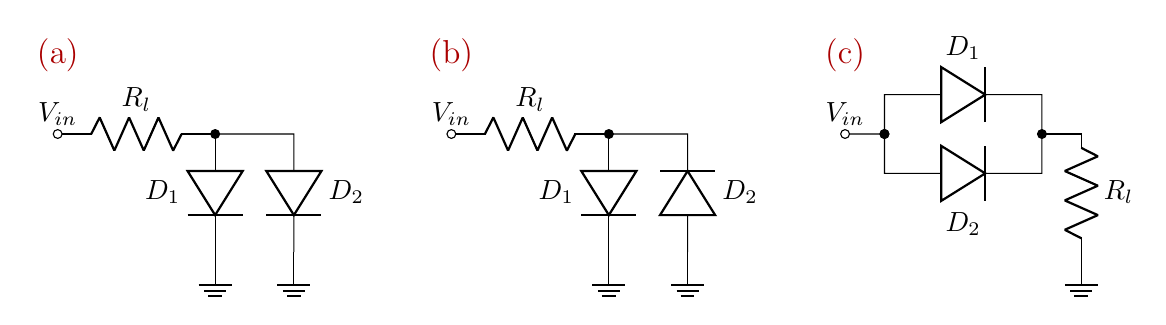
\begin{tikzpicture}
    \begin{scope}
        \node[anchor=center, color=myred, align=center] at (0, 1.0) {\large (a)};
        \node[anchor=center, align=center] at (0, 0.25) {$V_{in}$};
        \draw (0, 0)
            to[R, o-, l={$R_l$}] ++(2.0, 0)
            to[D, *-, l_={$D_1$}] ++(0.0, -1.5)
            node[ground] {};
        \draw (2.0, 0)
            to[short] ++(1.0, 0)
            to[D, l={$D_2$}] ++(0.0, -1.5)
            node[ground] {};
    \end{scope}
    \begin{scope}[xshift=5cm]
        \node[anchor=center, color=myred, align=center] at (0, 1.0) {\large (b)};
        \node[anchor=center, align=center] at (0, 0.25) {$V_{in}$};
        \draw (0, 0)
            to[R, o-, l={$R_l$}] ++(2.0, 0)
            to[D, *-, l_={$D_1$}] ++(0.0, -1.5)
            node[ground] {};
        \draw (2.0, 0)
            to[short] ++(1.0, 0)
            to[D, l={$D_2$}, invert] ++(0.0, -1.5)
            node[ground] {};
    \end{scope}
    \begin{scope}[xshift=10cm]
        \node[anchor=center, color=myred, align=center] at (0, 1.0) {\large (c)};
        \node[anchor=center, align=center] at (0, 0.25) {$V_{in}$};
        \draw (0, 0)
            to[short, o-*] ++(0.5, 0)
            to[short, *-] ++(0, 0.5)
            to[D, l={$D_1$}] ++(2.0, 0)
            to[short, -*] ++(0, -0.5);
        \draw (0.5, 0)
            to[short] ++(0, -0.5)
            to[D, l_={$D_2$}] ++(2.0, 0)
            to[short] ++(0, 0.5);
        \draw (2.5, 0)
            to[short] ++(0.5, 0)
            to[R, l={$R_l$}] ++(0.0, -1.5)
            node[ground] {};
    \end{scope}
\end{tikzpicture}
\end{document}